\documentclass{beamer}

\usepackage{amsmath,amsfonts,amssymb}
\usepackage{graphicx}
\usepackage{tikz}

\title{How to Conduct Interdisciplinary Research}
\subtitle{Strategies for Integrating Knowledge Across Fields}
\author{Morten Hjorth-Jensen}
\date{March 24, 2026, DScience workshop}

\begin{document}

\frame{\titlepage}

%------------------------------------------------

\begin{frame}{Motivation}

Many of today's scientific challenges cannot be solved
within a single discipline.

Examples include

\begin{itemize}
\item climate modeling
\item artificial intelligence and neuroscience
\item quantum computing and materials science
\item computational biology
\item complex socio-technical systems
\end{itemize}

These problems require integrating knowledge
from multiple scientific fields.

\end{frame}

%------------------------------------------------

\begin{frame}{What is Interdisciplinary Research?}

Interdisciplinary research involves

\begin{itemize}
\item integrating knowledge from different disciplines
\item combining methodologies
\item creating shared conceptual frameworks
\end{itemize}

Important distinctions:

\begin{itemize}
\item \textbf{Multidisciplinary}: disciplines coexist
\item \textbf{Interdisciplinary}: disciplines interact
\item \textbf{Transdisciplinary}: new frameworks emerge
\end{itemize}

\end{frame}

%------------------------------------------------

\begin{frame}{Why Interdisciplinary Research Matters}

Benefits include

\begin{itemize}
\item solving complex scientific problems
\item generating innovative research directions
\item connecting theory, experiment, and computation
\item enabling technological innovation
\end{itemize}

Many breakthroughs occur at the intersection of fields.

\end{frame}

%------------------------------------------------

\begin{frame}{Example: Physics and Machine Learning}

Recent examples include

\begin{itemize}
\item neural-network quantum states
\item machine learning for phase transitions
\item physics-informed neural networks
\item AI-driven discovery of materials
\end{itemize}

These developments illustrate how methods from
computer science can accelerate physics research.

\end{frame}

%------------------------------------------------

\begin{frame}{Example: Physics and Neuroscience}

Statistical physics has influenced neuroscience.

Examples include

\begin{itemize}
\item Hopfield networks and spin models
\item neural population dynamics
\item collective behavior in neural systems
\item connectome network analysis
\end{itemize}

This interaction has helped build theoretical
frameworks for understanding brain function.

\end{frame}

%------------------------------------------------

\begin{frame}{Example: Quantum Technology and AI}

Another emerging intersection is

\begin{itemize}
\item reinforcement learning for quantum control
\item machine learning for quantum error correction
\item quantum machine learning algorithms
\item hybrid quantum–classical optimization
\end{itemize}

These areas illustrate how interdisciplinary research
creates entirely new fields.

\end{frame}

%------------------------------------------------

\begin{frame}{Interdisciplinary Collaboration Network}

\begin{center}

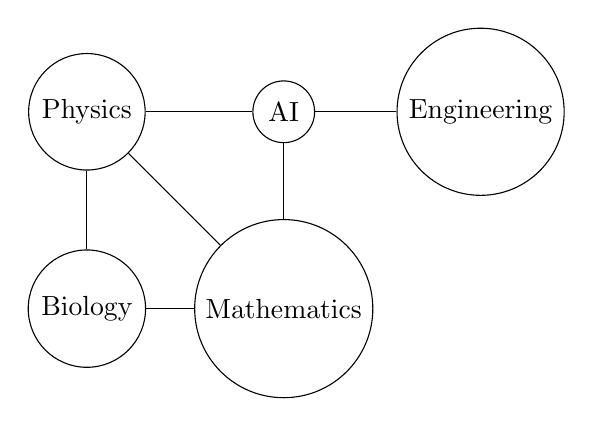
\begin{tikzpicture}[node distance=2.5cm]

\node (physics) [draw, circle] {Physics};
\node (ai) [draw, circle, right of=physics] {AI};
\node (bio) [draw, circle, below of=physics] {Biology};
\node (math) [draw, circle, below of=ai] {Mathematics};
\node (eng) [draw, circle, right of=ai] {Engineering};

\draw[-] (physics) -- (ai);
\draw[-] (physics) -- (bio);
\draw[-] (ai) -- (math);
\draw[-] (math) -- (bio);
\draw[-] (ai) -- (eng);
\draw[-] (physics) -- (math);

\end{tikzpicture}

\end{center}

Scientific breakthroughs often occur at the
intersections of these fields.

\end{frame}

%------------------------------------------------

\begin{frame}{Challenges in Interdisciplinary Research}

Common challenges include

\begin{itemize}
\item different scientific languages
\item different methodological traditions
\item communication barriers
\item differences in publication culture
\end{itemize}

These challenges require deliberate effort
to overcome.

\end{frame}

%------------------------------------------------

\begin{frame}{Building an Interdisciplinary Project}

Successful projects typically include

\begin{itemize}
\item a clearly defined scientific problem
\item complementary expertise
\item shared conceptual framework
\item collaborative infrastructure
\end{itemize}

The scientific problem should drive the collaboration.

\end{frame}

%------------------------------------------------

\begin{frame}{Developing a Shared Language}

Strategies include

\begin{itemize}
\item defining common terminology
\item identifying conceptual overlaps
\item documenting assumptions
\item encouraging cross-disciplinary learning
\end{itemize}

Communication is essential for successful collaboration.

\end{frame}

%------------------------------------------------

\begin{frame}{Designing Interdisciplinary Projects}

Key elements include

\begin{itemize}
\item defining clear research questions
\item combining complementary methodologies
\item establishing milestones
\item creating shared software and data resources
\end{itemize}

Good project management is crucial.

\end{frame}

%------------------------------------------------

\begin{frame}{Advice for PhD Students}

Students entering interdisciplinary research should

\begin{itemize}
\item build strong foundations in one field
\item develop literacy in neighboring disciplines
\item cultivate curiosity and openness
\item collaborate with diverse research groups
\end{itemize}

Interdisciplinary expertise develops gradually.

\end{frame}

%------------------------------------------------

\begin{frame}{Developing Interdisciplinary Skills}

Important skills include

\begin{itemize}
\item communication across disciplines
\item computational literacy
\item data analysis skills
\item collaborative project management
\end{itemize}

These skills are increasingly valued in academia
and industry.

\end{frame}

%------------------------------------------------

\begin{frame}{Publishing Interdisciplinary Research}

Possible venues include

\begin{itemize}
\item interdisciplinary journals
\item computational science journals
\item domain-specific journals with cross-disciplinary focus
\end{itemize}

Selecting the right audience is important.

\end{frame}

%------------------------------------------------

\begin{frame}{Writing Interdisciplinary Grant Proposals}

Key elements include

\begin{itemize}
\item clear scientific question
\item justification of interdisciplinary approach
\item complementary expertise of team members
\item impact beyond a single field
\end{itemize}

Funding agencies increasingly encourage
cross-disciplinary collaborations.

\end{frame}

%------------------------------------------------

\begin{frame}{Interdisciplinary Research Centers}

Many universities now establish

\begin{itemize}
\item interdisciplinary research centers
\item cross-department institutes
\item collaborative graduate programs
\end{itemize}

These structures facilitate collaboration
between fields.

\end{frame}

%------------------------------------------------

\begin{frame}{Common Pitfalls}

Typical problems include

\begin{itemize}
\item superficial integration of disciplines
\item unclear research goals
\item lack of shared conceptual framework
\item poor communication
\end{itemize}

Successful interdisciplinary research requires
intentional planning.

\end{frame}

%------------------------------------------------

\begin{frame}{Best Practices}

Successful interdisciplinary researchers

\begin{itemize}
\item maintain depth in a core discipline
\item collaborate broadly
\item remain intellectually curious
\item cultivate communication skills
\end{itemize}

Interdisciplinary work combines intellectual
depth with collaborative breadth.

\end{frame}

%------------------------------------------------

\begin{frame}{Conclusion}

Interdisciplinary research is increasingly essential
for addressing complex scientific challenges.

Success depends on

\begin{itemize}
\item integrating knowledge across fields
\item strong collaboration
\item shared conceptual frameworks
\end{itemize}

The future of scientific discovery will likely be
deeply interdisciplinary.

\end{frame}

\end{document}
